%======================================================================
\chapter{Procedure}
%======================================================================

The entire process from start to finish will be documented in the following chapter, alongside subsections for each step. To begin, a high-level overview of the generation pipeline will be discussed, followed by a more technical breakdown of what each of the three major stages entail. 

\hfill

To start, \autoref{figure:architecture} demonstrates the system architecture, which is broken down into the environment setup, generation pipeline, and regeneration pipeline steps. Since the first and third components play a lesser role throughout the project, they will only be discussed briefly, while the second component will be the primary focus of this chapter.

\hfill

\begin{figure}[hbt]
  \centering
  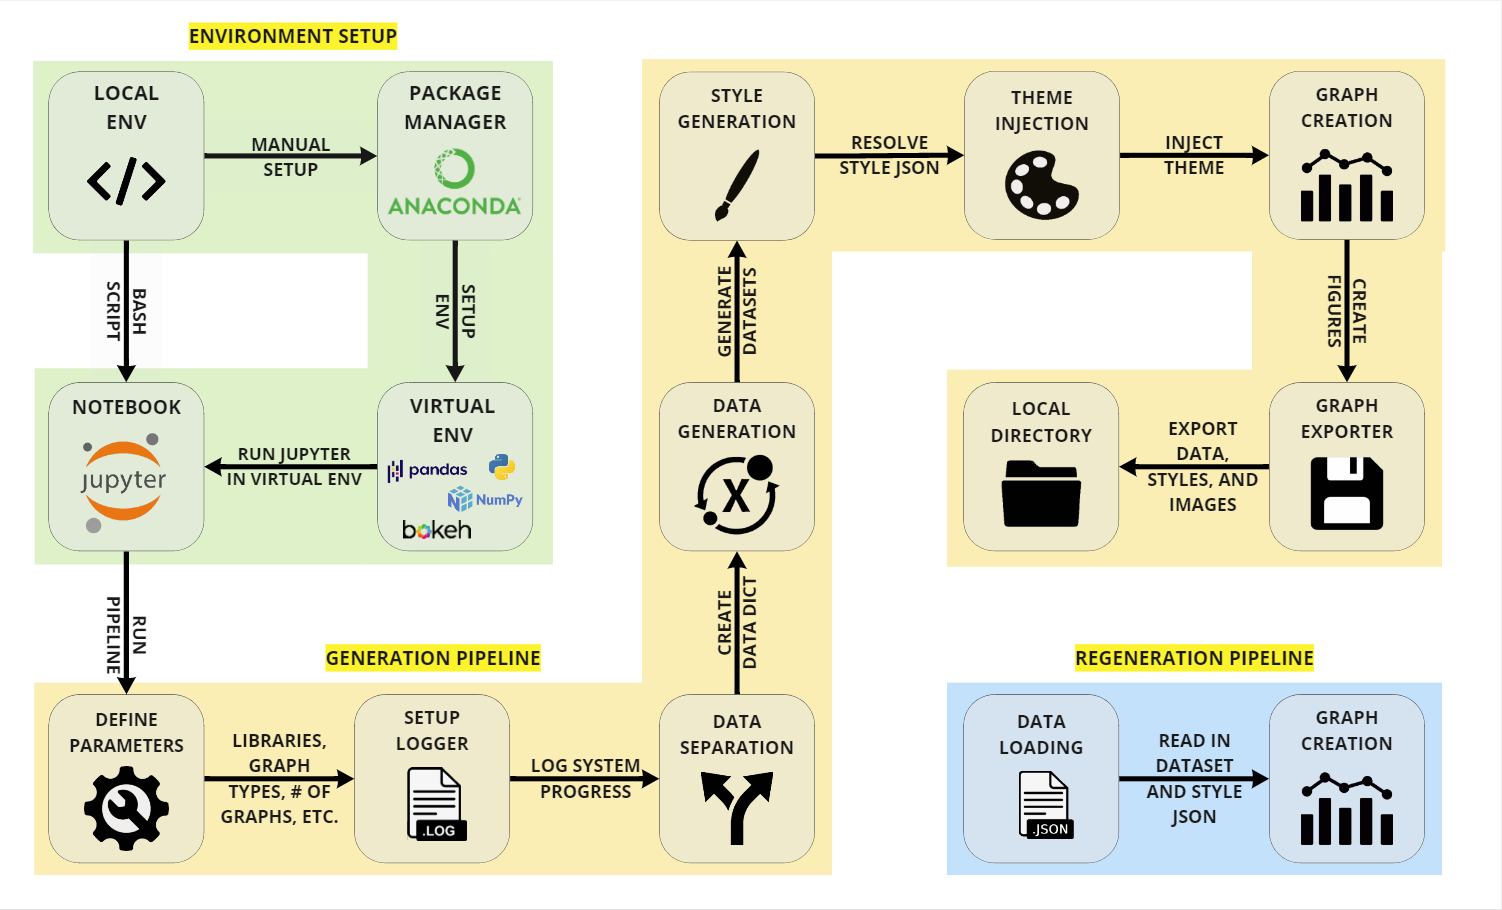
\includegraphics[width=\textwidth,height=\textheight,keepaspectratio]{figures/body/procedure/architecture_diagram}
  \caption{Graph generation system architecture}
\label{figure:architecture}
\end{figure}

\section{Environment Setup}

The environment setup stage is tasked with setting up the development environment as well as all required dependencies and packages. An essential part of this step is that the target system must contain both
\href{https://www.anaconda.com/}{Anaconda} as well as some sort of interactive Python command shell such as \href{https://ipython.org/}{iPython}, \href{https://jupyter.org/}{Jupyter}, or \href{https://research.google.com/colaboratory/}{Google Colab}. Jupyter was used for the development of this project, which is the interactive Python environment that will be described going forward. 

\hfill

Once all the required dependencies are installed, the first step is to utilize Anaconda, the de facto standard for Python package distribution. It will be used to create a virtual environment in the target location. This environment will house all of the required packages in an environment separate from the system and any other projects. This is largely to avoid compatibility issues between sharing libraries, as well as promote reproducible development environments. The setup of this virtual environment will also include the download and installation of required software such as \href{https://www.python.org/}{Python}, \href{https://numpy.org/}{NumPy}, \href{https://pandas.pydata.org/}{pandas}, \href{https://bokeh.org/}{Bokeh}, \href{https://altair-viz.github.io/}{Altair}, and \href{https://plotnine.readthedocs.io/en/stable/}{plotnine} amongst others. The file containing all required dependencies as well as their specified versions can be found at \path{setup/environment.yml}. Upon successful installation, the final step is to launch the Jupyter environment, also known as an interactive Python notebook. This notebook will be used to execute the code in a linear fashion while maintaining variables between code blocks and allow for inline documentation through markdown text styling.

\hfill

A custom \href{https://www.gnu.org/software/bash/}{Bash} script was made to automate the entire environment setup using as a little as a standard computer terminal. The automation takes care of everything from the initial environment creation up until running the Jupyter notebook, which will need to be executed by a user. It is worth mentioning that the script (\path{setup/setup.sh}) is compatible with both MacOS and Unix based devices, however, it is not recommended for use on Windows-based machines.

\section{Generation Pipeline}
The generation pipeline was the core development that was undertaken, and acts as the backbone for the entire project. It includes everything from generating a list of how many graphs per library are required to the exporting of individual graphs.

\hfill

As seen in \autoref{figure:plots}, the generation process contains a multitude of steps, however, only a few of the critical steps will be brushed on in the coming subsections. Namely, the data separation, data generation, style generation, graph creation, and graph exportation stages will be covered, as they play the most crucial roles and are less self explanatory than others.

\subsection{Data Separation}
\label{subsection:data_separation}
Data separation begins with the pipeline's hyperparameters. These include the number of graphs to generate, as well as the graph types and libraries to generate from. An additional exclusion parameter is specified to ignore any graph-library combinations. One such example would be Altair-based contour plots, as they are not supported by the library's rendering engine.

\hfill

The data separation step then utilizes these hyperparameters to generate an occurrence dictionary, which represents the number of graphs that should be generated for each graph-library pair. There are optional flags for forcing a randomized distribution between graph types as well as libraries, however, this approach is not recommended as certain combinations may not be selected, thus generating a dataset of lower variance and potentially higher bias.

\hfill 
\newcolumntype{P}[1]{>{\centering}p{#1\textwidth}}

\begin{table}[!ht]
    \centering
    \begin{tabular}{p{0.2\textwidth}P{0.1}P{0.1}P{0.1}P{0.1}P{0.1}>{\arraybackslash}P{0.1}}\toprule
        \multirow{2}{*}{\textbf{Graph Type}}&\multicolumn{3}{c}{\textbf{Library (Equal)}}&\multicolumn{3}{c}{\textbf{Library (Random)}}\\
        & Bokeh & Altair & plotnine & Bokeh & Altair & plotnine\\
        \midrule
        Area Graph & 5 & 5 & 4 & 1 & 4 & 9\\
        Bar Chart & 5 & 5 & 4 & 0 & 4 & 1\\
        Box Plot & 5 & 4 & 4 & 6 & 0 & 3\\
        Bubble Plot & 5 & 5 & 4 & 0 & 0 & 0\\
        Contour Plot & 5 & 5 & 4 & 0 & 0 & 0\\
        Error Bar & 5 & 4 & 4 & 13 & 1 & 5\\
        Histogram & 5 & 5 & 4 & 1 & 4 & 1\\
        KDE Plot & 5 & 5 & 4 & 0 & 0 & 5\\
        Line Graph & 5 & 4 & 4 & 52 & 7 & 33\\
        Scatter Plot & 5 & 5 & 4 & 0 & 0 & 0\\
        Violin Plot & 5 & 4 & 4 & 0 & 0 & 0\\
        \bottomrule
    \end{tabular}
    \caption{Graph-type to library occurrences (150) for equal and random distributions}
\end{table}

\subsection{Data Generation}
\label{subsection:data_generation}
The data generation process is arguably the most important process of the entire project. Acting as a middleware service between the data separation and creation steps, it takes the aforementioned occurrence dictionary as input and generates a new dictionary containing the generated graph objects, binning each based on graph type. Each bin stores an array of graph objects with their respective IDs, specified creation library, and generated data. 

\hfill

The data produced in this step typically include a set of \(X\) and \(y\) data points, however, certain graph-types may require information such as the type of distribution, number of layers, bubble sizes, \(z\) values, and correlation type (\autoref{figure:example_data_json}). These values are specified based on graph type and the generation for which can be found in the \path{generators} directory. It should be noted that each Python file (\path{.py}) in the \path{generators} is named based on graph type and contains a required \path{generate_data()} function responsible for the data generation. Methodologies behind the various generation techniques are explained thoroughly in \autoref{chapter:methodology}. It should also be noted that data of any type and quantity can be provided to the generated object, as it will be used later in the creation and exportation steps.

\hfill

After sequentially generating the data for each individual graph, this master dictionary is then supplied to the ``stylizer" for both style generation and theme injection.

\begin{figure}
    \begin{minted}[frame=single,
                   framesep=3mm,
                   linenos=true,
                   xleftmargin=21pt,
                   baselinestretch=0.8,
                   tabsize=4]{js}
{
    "X": [
        "A",
        "B",
        ...
    ],
    "y": [
        6.253763991874621,
        13.491181938914046,
        12.86460662847583,
        ...
    ],
    "is_vertical": false,
    "correlation": "positive"
}
    \end{minted}
    \caption{Example of a bar chart data generation object} 
    \label{figure:example_data_json}
\end{figure}

\subsection{Style Generation}
\label{subsection:style_generation}
The primary role of the stylization module is to generate styles for a given library-graph pair. Taking in both the graph type and library type, the styles are generated on the fly for each individual graph in the form of a key-value dictionary. An additional input parameter is specified containing the number of repeated styles, if any, that need to be generated. This is beneficial for graphs that require multiple styles based on the size and shape of the dataset. For instance, area plots typically contain a multitude of layers and may require a different colour for each layer.

\hfill

These style dictionaries are generated by reading in the \path{JSON} document from the \path{styles} directory and parsing the corresponding style document. Each file is named based on graph type (i.e. \path{scatter.json}) and contains a \path{default} property as well an object property for each respective visualization library (i.e. \path{bokeh}, \path{altair}, etc.). These properties contain objects representing the styles that should be given to each or all of the functions responsible for plotting the graphs. Specifically, the values contain a structure similar to \autoref{figure:example_style_json}, where the key denotes the property name and the value represents an object containing type and value fields. The type field mentioned above specifies how the value should be resolved and the value field is used as input for that resolution. These property objects are then used by the style resolver, whose details will be covered in the following paragraph.

\begin{figure}
    \begin{minted}[frame=single,
                   framesep=3mm,
                   linenos=true,
                   xleftmargin=21pt,
                   baselinestretch=0.8,
                   tabsize=4]{js}
{     
    "default": {
        "line_color": {
            "type": "color",
            "repeat": true
        }
    },
    "bokeh": {
        "line_thickness": {
            "type": "range",
            "value": [0.4, 0.8],
            "float": true
        }
    },
    ...
}
    \end{minted}
    \caption{Example of a line graph's stylization JSON file} 
    \label{figure:example_style_json}
\end{figure}

These properties are then passed to a style resolver, which resolves styles from the input object to usable values. For instance, this may turn a colour field into a usable hex color code, randomly generate a value between a specified range, or select a single item from a list of options. In addition to the above, the style resolver supports generating random booleans, reading in \path{JSON} file paths, and returning static values. These resolutions are defined in a dictionary that maps style types to their respective functions. Any additional parameters the style object possesses will be passed down to the corresponding resolve function. This has many uses cases such as indicating whether a field should be repeated, or whether a value should return a float.

\hfill

After resolving each style to the correct value, a random theme is selected based on library type. Both the chosen theme's name and newly generated styles are attached to the graph object currently being iterated over. This completed data object is then supplied to the graph creation step for image production.

\subsection{Graph Creation}
The graph creation takes in the previously generated data and styles and outputs a graph using the corresponding visualization library. The architecture for this is not unlike the graph generation process, where each Python file (\path{.py}) in the \path{creators} directory contains a function for every graphing library (i.e. \path{create_bokeh_graph()}, \path{create_altair_graph()}, etc.). Prior to graph creation, any initialization functions, known as pre-creation hooks, are executed. Following, the theme is set for the visualization libraries in a process known as theme injection.

\begin{figure}
    \centering
    \begin{subfigure}[b]{0.32\textwidth}
        \centering
        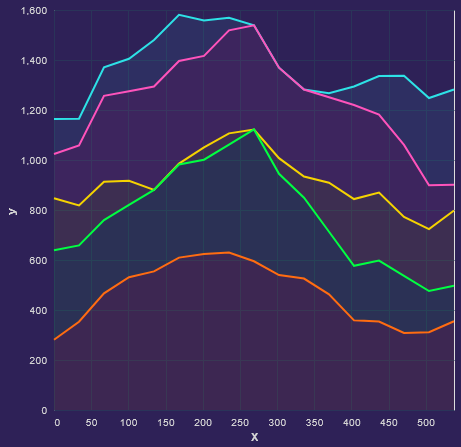
\includegraphics[width=\textwidth]{figures/body/procedure/area.png}
    \end{subfigure}
    \hfill
    \begin{subfigure}[b]{0.32\textwidth}
        \centering
        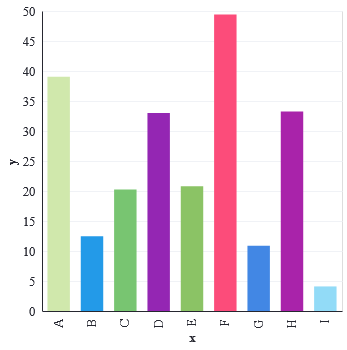
\includegraphics[width=\textwidth]{figures/body/procedure/bar.png}
    \end{subfigure}
    \hfill
    \begin{subfigure}[b]{0.32\textwidth}
        \centering
        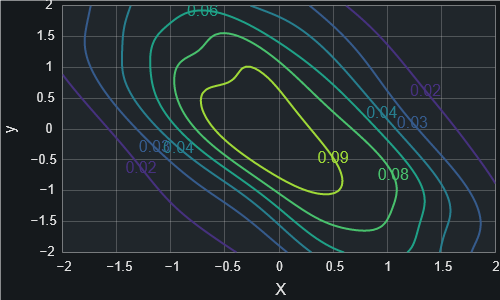
\includegraphics[width=\textwidth]{figures/body/procedure/contour.png}
    \end{subfigure}
    \centering
    \begin{subfigure}[b]{0.32\textwidth}
        \centering
        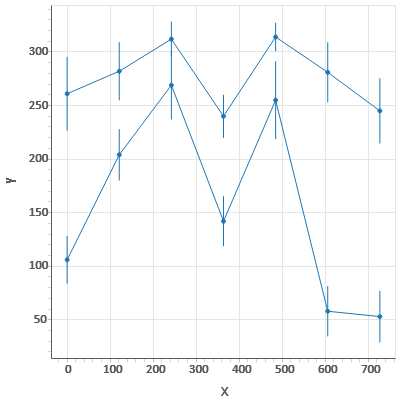
\includegraphics[width=\textwidth]{figures/body/procedure/error.png}
    \end{subfigure}
    \hfill
    \begin{subfigure}[b]{0.32\textwidth}
        \centering
        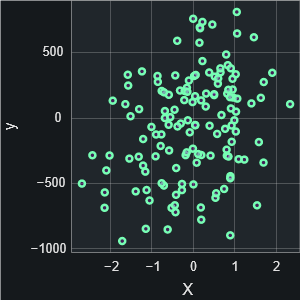
\includegraphics[width=\textwidth]{figures/body/procedure/scatter.png}
    \end{subfigure}
    \hfill
    \begin{subfigure}[b]{0.32\textwidth}
        \centering
        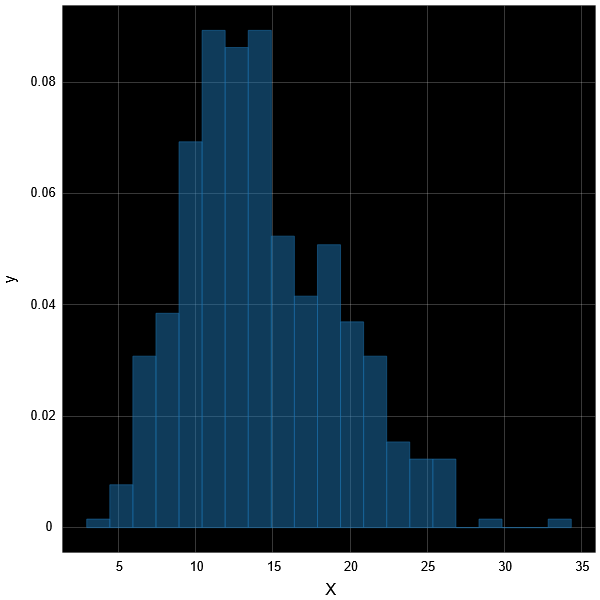
\includegraphics[width=\textwidth]{figures/body/procedure/hist.png}
    \end{subfigure}
    \centering
    \begin{subfigure}[b]{0.32\textwidth}
        \centering
        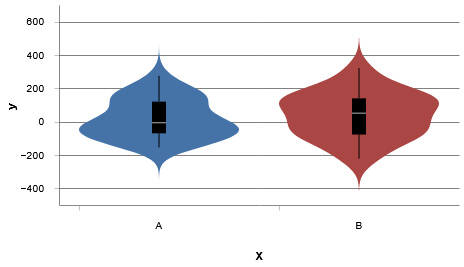
\includegraphics[width=\textwidth]{figures/body/procedure/violin.png}
    \end{subfigure}
    \hfill
    \begin{subfigure}[b]{0.32\textwidth}
        \centering
        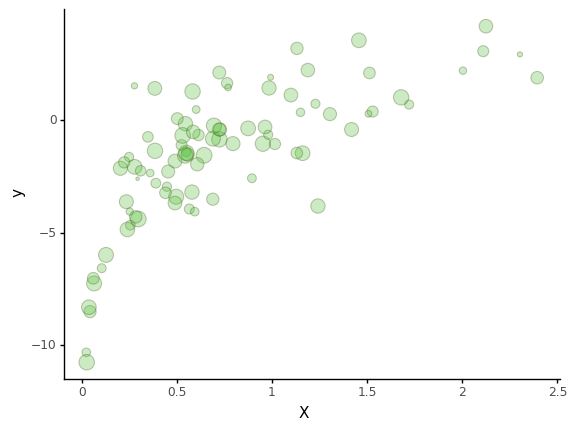
\includegraphics[width=\textwidth]{figures/body/procedure/bubble.png}
    \end{subfigure}
    \hfill
    \begin{subfigure}[b]{0.32\textwidth}
        \centering
        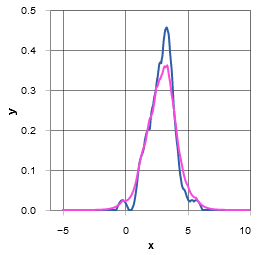
\includegraphics[width=\textwidth]{figures/body/procedure/kd.png}
    \end{subfigure}
    \caption{Various plots with random styles and themes generated using the pipeline}
    \label{figure:plots}
\end{figure}

This process involves retrieving the theme name from the generated data and reading in the corresponding theme file which is then injected into the generated graph. Should the visualization library require this to occur after graph generation, a post-creation hook is provided. The injection is the process of injecting usable theme data into the graph for stylization purposes. 

\hfill 

More technically, each file in the \path{libraries} directory possesses a name corresponding to the desired visualization library, and contains a single Python class. These \path{Library} classes contain the functions for setup, pre-creation, post-creation, theme setting, and graph exportation, with the latter being discussed in \autoref{subsection:graph_exportation}.

\subsection{Graph Exportation}
\label{subsection:graph_exportation}
Graph exportation is the process of exporting the data, styles, and image of a particular graph to local storage. The data and styles are stored as separate \path{JSON} files in the \path{output/data} and \path{output/styles} directories respectively. The images, however, are stored in Portable Network Graphics (\path{.PNG}) format at the \path{output/images} directory. All three of the graph's output files are saved using the same \path{type_library_id} naming convention, where type and library represent the graph type and visualization library respectively. The graph ID on the other hand, represents the current number in the sequence of graphs with identical graph-types and libraries. For instance, the naming convention may be seen as \path{area_bokeh_0} followed by \path{area_bokeh_1} and \path{area_altair_0}. 

\hfill

Since the graph content can be exported, the data and style objects need to be serialized into a JSON-compatible format. This serialization process involves turning values such as NumPy arrays or pandas DataFrames into standard Python lists. The provided values are serialized based on type, and recursion is used to serialized nested values such as 2-D or 3-D arrays. Once serialized, the data, styles, and images are ready to be exported. Graph exportation is a crucial aspect of the project as it allows for graph regeneration, which is essential for determining model correctness and will be covered in \autoref{section:regeneration_pipeline}.

\section{Regeneration Pipeline}
\label{section:regeneration_pipeline}
The regeneration pipeline is tasked with regenerating graphs from two input sources, namely the data and styles objects, and is a critical aspect of the project. As the pipeline above will be involved in creating input data for a Generative Adversarial Network (GAN), it is necessary to compare the images from both the original pipeline, as well as the GAN, in order to assess network accuracy.

\subsection{Chart Regeneration}
\label{subsection:chart_regeneration}
The chart regeneration process was designed to be run as a standalone process and as such, begins by running any required library setup. Following, the \path{data} and \path{styles} folders in the \path{ingestion} directory are intersected to find all valid graphs. Once a valid graph list is made, the same code used for graph creation can be run on the read-in data and style objects. However, the data must be de-serialized as it is being read-in and not exported like mentioned in \autoref{subsection:graph_exportation}. This involves reversing the previous serialization procedure by converting values from their basic Python classes to more appropriate instances, such as a primitive list object to a NumPy array.

\hfill

Once de-serialization is complete, the data is ready to be used for graph creation. This involves passing the content to the graph creation process one at a time, just like the original creation process. During this graph regeneration, the images are outputted to the \path{ingestion/images} directory in PNG format, using the same filename as the inputted data and style files.

%----------------------------------------------------------------------
